\documentclass[11pt,twoside]{article}
% \input{hwheader.tex}

%\documentclass[11pt,twoside]{article}
\usepackage[nonamelimits]{amsmath}
\usepackage{amssymb, amsthm}

\setlength{\oddsidemargin}{0 in}
\setlength{\evensidemargin}{0 in}
\setlength{\topmargin}{-0.6 in}
\setlength{\textwidth}{6.5 in}
\setlength{\textheight}{8.5 in}
\setlength{\headheight}{0.5 in}
\setlength{\headsep}{0.5 in}
\setlength{\parindent}{0 in}
\setlength{\parskip}{0.1 in}

%%% SETS
\newcommand\Z{\mbox{$\mathbb Z$}}
\newcommand\N{\mbox{$\mathbb N$}}
\newcommand\R{\mbox{$\mathbb R$}}
\newcommand\F{\mbox{$\mathbb F$}}
\def\B{\{0,1\}}
\def\cond{\mid}

%%% FUNCTIONS
\providecommand\floor[1]{\lfloor#1\rfloor}
\providecommand\ceil[1]{\lceil#1\rceil}
\providecommand\blog[1]{\log_2\ceil{#1}}
\providecommand\abs[1]{\lvert#1\rvert}
\providecommand\bigabs[1]{\bigl\lvert#1\bigr\rvert}

\def\co{{\rm co}}
\def\avg{{\rm Avg}}
\def\heur{{\rm Heur}}

%%% THEOREM TYPE ENVIRONMENTS
\newtheorem{theorem}{Theorem}
\newtheorem{lemma}[theorem]{Lemma}
\newtheorem{corollary}[theorem]{Corollary}
\newtheorem{proposition}[theorem]{Proposition}
\newtheorem{claim}[theorem]{Claim}
\newtheorem{exercise}{Exercise}
\newtheorem{conjecture}{Conjecture}
\newtheorem{example}{Example}
\newtheorem{remark}{Remark}
\newtheorem{definition}[theorem]{Definition}

%%% HEADINGS
\newcommand{\homework}[1]{
   \pagestyle{myheadings}
   \thispagestyle{plain}
   \newpage
   \setcounter{page}{1}
   \noindent
   \classname \hfill \mbox{\updatedday} \\
   \instname \hfill \mbox{\duedate}
   \rule{6.5in}{0.5mm}
   \vspace*{-0.1 in}
}


\newcommand{\problem}[1]{\section*{Problem #1}}


\renewcommand{\labelenumi}{(\alph{enumi})}
\renewcommand{\labelenumii}{(\roman{enumii})}

%%% DEFINITIONS
\def\classname{CSCI-SHU 2314: Discrete Math}


%%% INSTRUCTIONS
\raggedbottom 


\usepackage[pdftex]{graphicx}
\usepackage{pgf,tikz}
\usetikzlibrary{shapes,arrows,automata}

\usepackage{listings}
\usepackage{xcolor}
\lstset { %
    language=C++,
    backgroundcolor=\color{black!5}, % set backgroundcolor
    basicstyle=\footnotesize,% basic font setting
}

\newcommand\includefa[1]{\begin{center}\includegraphics[scale=0.5]{#1}\end{center}}

\def\updatedday{Posted: November 25, 2024}
\def\duedate{Due: 11:30pm (Shanghai time), December 10, 2024}
\newenvironment{solution}{{\par\noindent\it Solution.}}{}

\def\instname{Homework 4}

\pagenumbering{gobble}

\begin{document}
\homework{1}

This assignment has in total $100$ base points and $20$ bonus points, and the cap is $100$.
Bonus questions are indicated using the $\star$ mark.

\textit{Please specify the following information before submission}:
\begin{itemize}
    \item Your Name: %  (put your name here)
    \item Your NetID: % (put your NetID here)
\end{itemize}



\problem{1: Combinatorial proofs [10+10 pts]} 

Give combinatorial proofs for the following equalities.

\begin{enumerate}

    \item $\binom{n}{1}-2\binom{n}{2}+3\binom{n}{3}+\cdots+(-1)^{n-1}\cdot n \binom{n}{n} = 0$
    \item $\binom{n}{m} \binom{r}{0} + \binom{n-1}{m-1} \binom{r+1}{1} + \binom{n-2}{m-2} \binom{r+2}{2} +\cdots+ \binom{n-m}{0} \binom{r+m}{m} = \binom{n+r+1}{m}$
    
\end{enumerate}

\hspace*{\fill}

Pf:

(a)

LHS $=\binom{n}{1}-2\binom{n}{2}+3\binom{n}{3}+\cdots+(-1)^{n-1}\cdot n \binom{n}{n} = \sum ^n_ {i=1} (-1)^{i-1}i C^i_n$

Note that: $iC^i_n = i\cfrac{n!}{i!(n-i)!} = \cfrac{n(n-1)!}{(i-1)!(n-i)!} = nC^{i-1}_{n-1}$

Therefore, LHS $= \sum ^n_ {i=1} (-1)^{i-1}nC^{i-1}_{n-1} = n\sum ^n_ {i=1} (-1)^{i-1}C^{i-1}_{n-1}$

As already learnt in Xue's lecture 18: $\sum ^n_ {k=0} (-1)^{k}C^{k}_{n} = 0$

Hence, LHS $=0\cdot n=0=$ RHS

QED




\problem{2: Number of intersection points [20 pts]}
Consider a disk $D$ in the plane.
Let $S$ be a set of $n$ (different) points on the boundary of $D$.
For every $a,a' \in S$ with $a \neq a'$, we connect $a$ and $a'$ by a segment $\mathsf{seg}(a,a')$.
Suppose that for any different points $a,a',b,b',c,c' \in S$, the three segments $\mathsf{seg}(a,a')$, $\mathsf{seg}(b,b')$, and $\mathsf{seg}(c,c')$ do \textit{not} intersect at a common point.
Our goal is to count the intersection points of these segments \textit{inside the interior of the disk} (that means the points in $S$ are not considered as intersection points).
Let $f(n)$ be the number of such intersection points.
Give a formula for $f(n)$ and prove its correctness.
The figure below shows that $f(5) = 5$.

\begin{center}
    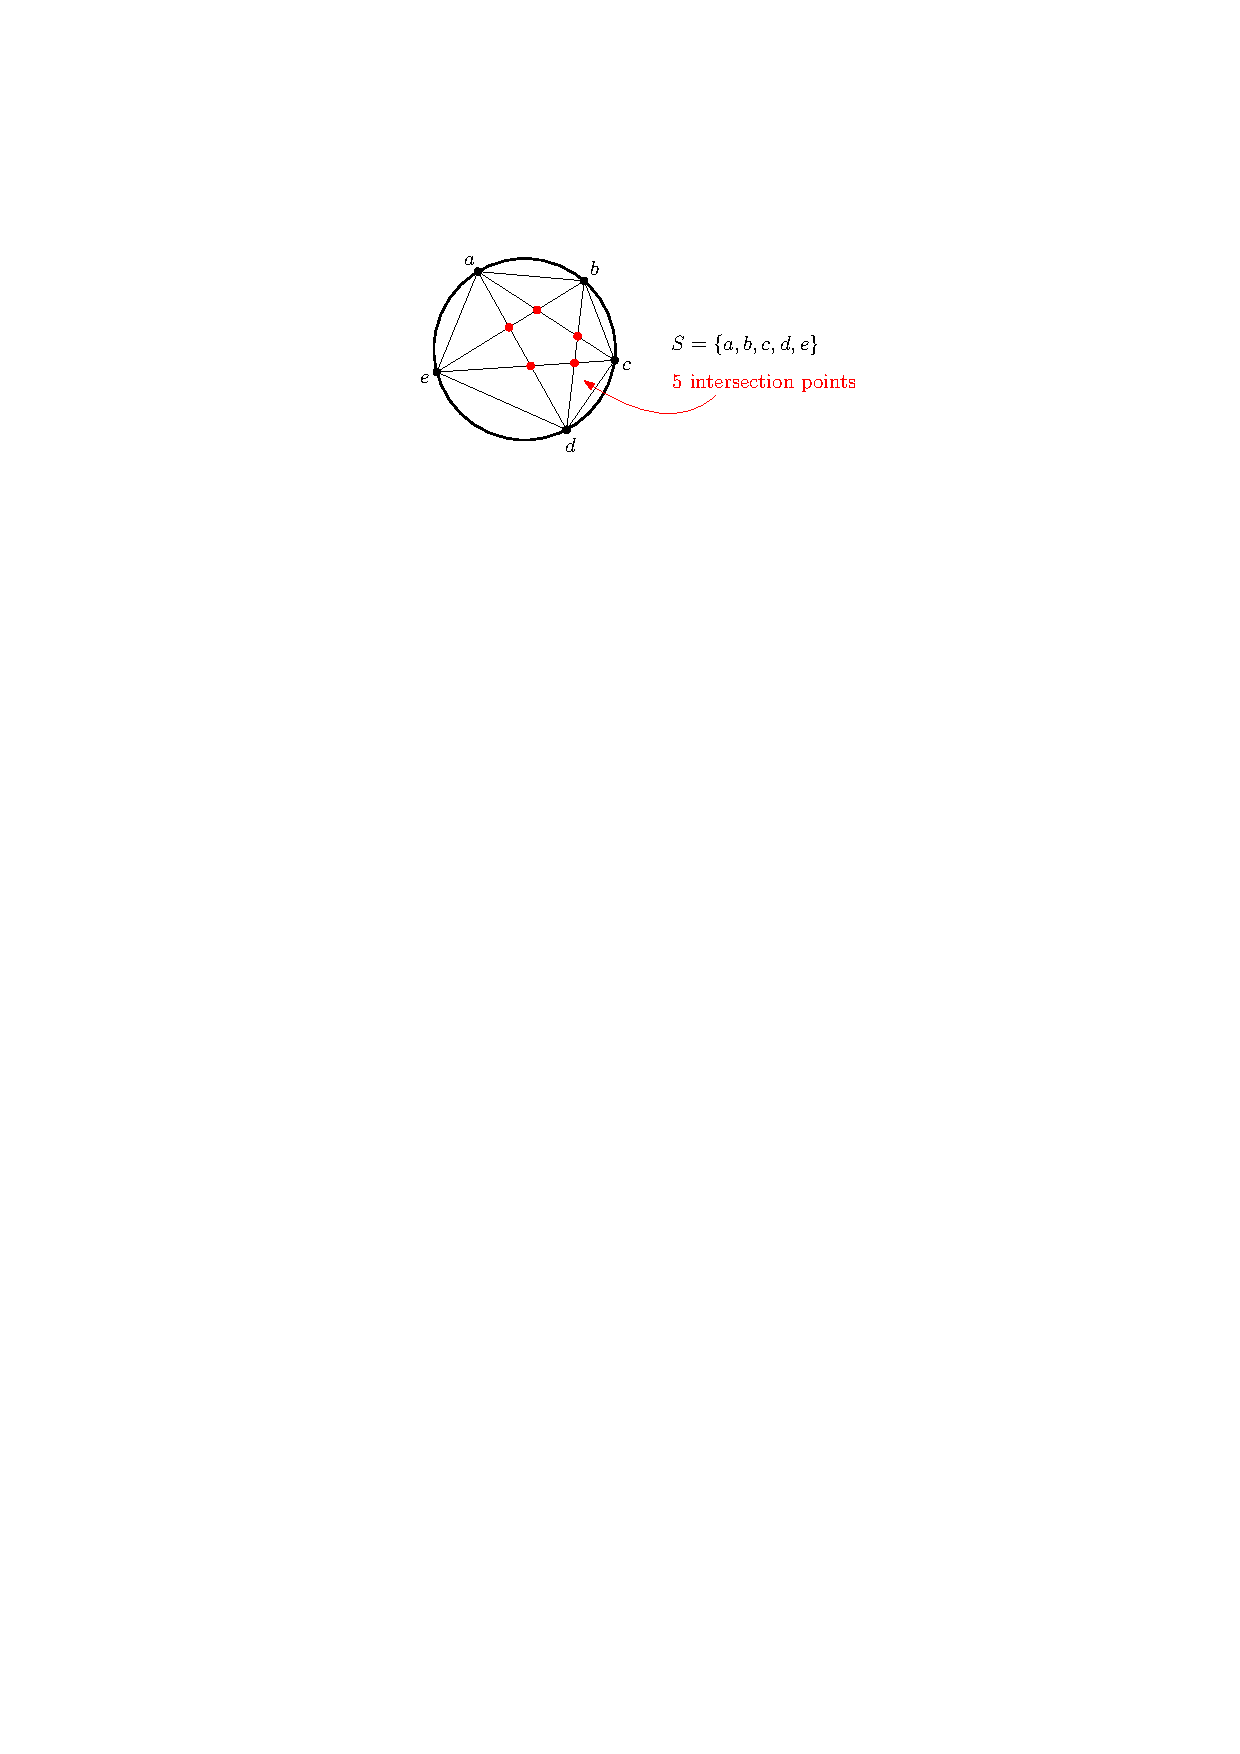
\includegraphics[height=5cm]{hw-fig-intersection.pdf}
\end{center}

\problem{3: Counting solutions [20 pts]}
Let $n,s,k \in \mathbb{N}$.
Consider the equation $x_1+x_2+\cdots+x_n = s$, where $x_1,\dots,x_n$ are variables.
We want to count the solutions to this equation satisfying that $x_i \in \{0,1,\dots,k\}$ for all $i$.
Prove that the number of such solutions is equal to $\binom{s+n-1}{n-1} - \sum_{i=1}^n (-1)^{i-1} \binom{n}{i} \binom{s-ik+n-1}{n-1}$.

\hspace*{\fill}

Pf:

As learnt in the Xie's recitation: the number of solutions of the equation $x_1+x_2+\cdots+x_n = s$, where $x_1,\dots,x_n$ are non-negative integers is $C^{n-1}_{s+n-1}$

Now suppose the number of $x_i$ s.t. $x_i > k $ is $m$

If we replace $y_i = x_i - k$, the equation becomes $y_1+y_2+\cdots+y_n = s-m(k+1)$, we can still use this formula

Therefore, the number of the solution satisfying $x_i \leq k$ is $C^{n-1}_{s-m(k+1)+n-1}$

And we also need to choose those $xi$ that greater than k, whose number is $C^m_n$

Hence, the total numbers of ways of solution in this situation is $C^m_nC^{n-1}_{s-m(k+1)+n-1}$

Note that the number of solutions to this equation satisfying that $0\leq x_i \leq k$ for all $i$ is those satisfying $0\leq x_i$ for all $i$ exclude those $\exists x_i > k$ for some $i$

By using the property of inclusion-exclusion, the number of solutions of the equation $x_1+x_2+\cdots+x_n = s$, where $x_1,\dots,x_n$ are non-negative integers and smaller than $k+1$ is exactly

$C^{n-1}_{s+n-1}-\sum ^n_{i=1} (-1)^{i-1 } C^i_nC^{n-1}_{s-i(k+1)+n-1}$

QED


\problem{4: Doubling sequences [20 pts]} 
We say a sequence $(a_1,\dots,a_k)$ of positive integers is a \textit{doubling sequence} if $a_i \geq 2a_{i-1}$ for all $i \in \{2,3,\dots,k\}$.
We want to count the doubling sequences whose last element is equal to a given number.
Formally, for a positive integer $n$, let $f(n)$ denote the number of doubling sequences (of any length) ending with $n$.
For example, we have $f(5) = 4$, since there are $4$ doubling sequences ending with $5$, namely, $(5)$, $(1,5)$, $(2,5)$, and $(1,2,5)$.
Prove that $f(n) = f(n-1) + \alpha(n) \cdot f(\lfloor n/2 \rfloor)$, where $\alpha(n) = 0$ if $n$ is odd and $\alpha(n) = 1$ if $n$ is even.

\problem{5: Nice colorings of a disk [10+10 pts]} 
We have a disk that is equally divided into $n$ sectors around the disk center.
The $n$ sectors are labeled by $0,1,\dots,n-1$ in clockwise order.
See the figure below.
We want to color these sectors using paints.
Suppose there are paints with $k$ different colors.
Each sector should be colored with one of these $k$ colors.
In addition, in order to make the disk have a good appearance, adjacent sectors are required to have \textit{different} colors.
A way to color the sectors under this constraint is called a \textit{nice $k$-coloring} of the disk.
Our goal is to compute the number of nice $k$-colorings.
Let $\textsc{Paint}_k(n)$ denote the number of nice $k$-colorings of a disk with $n$ sectors.
\begin{enumerate}
    \item Prove that $\textsc{Paint}_k(n) + \textsc{Paint}_k(n-1) = k(k-1)^{n-1}$.
    \item Based on the result of (a), further prove that $\textsc{Paint}_k(n) = k \sum_{i=1}^{n} (-1)^{i-1} (k-1)^{n-i}$.
\end{enumerate}

\begin{center}
    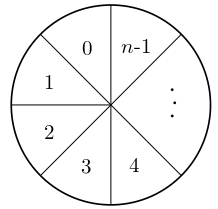
\includegraphics[height=5cm]{hw-fig-sector.jpg}
\end{center}

\problem{6: Bonus questions [20$^\star$ pts]}

{\color{red} You only need to select ONE of the following two problems to solve.
Solving both does not give you extra credits.
Please indicate clearly which problem you select.}

\begin{enumerate}
    \item This problem is an extension of Problem~5 above.
    In Problem~5, we have seen how to coumpute the number $\textsc{Paint}_k(n)$ of nice $k$-colorings of a disk with $n$ sectors.
    In this problem, we consider the setting where we can \textit{rotate} the disk.
    We say two colorings are \textit{equivalent} if one can rotate the disk to obtain one coloring from the other.
    Our goal is to compute the number of \textit{non-equivalent} nice $k$-colorings.
    Let $\textsc{Paint}_k^*(n)$ be the number of non-equivalent nice $k$-colorings of a disk with $n$ sectors.
    Prove that
    \begin{equation*}
        \textsc{Paint}_k^*(n) = \frac{\sum_{i=0}^{n-1} \textsc{Paint}_k(n/\mathsf{gcd}(n,i))}{n},
    \end{equation*}
    where $\mathsf{gcd}(n,i)$ is the greatest common divisor of $n$ and $i$.
    
    \item You have $n$ lockboxes $L_1,\dots,L_n$ and $n$ keys $K_1,\dots,K_n$, where the key $K_i$ can be used to open the lockbox $L_i$ (but not the other lockboxes).
    Let $m \in \{1,\dots,n\}$ be a number.
    Imagine that you and your friend are playing a game as follows.
    You keep the keys $K_1,\dots,K_m$ in your pocket and put the remaining keys $K_{m+1},\dots,K_n$ inside the lockboxes $L_1,\dots,L_n$ such that each lockbox contains at most one key.
    Clearly, there are $n!/m!$ different ways to put these $n-m$ keys.
    After this, your friend will close (and lock) all lockboxes.
    Now you are going to use the keys you have, $K_1,\dots,K_m$, to open the lockboxes $L_1,\dots,L_m$, get the keys inside these lockboxes, use them to open more lockboxes, get more keys, and so forth.
    You win the game if you can eventually open all lockboxes and obtain all keys.
    Prove that there are $(n-1)!/(m-1)!$ different ways to put the keys for which you can win the game.
\end{enumerate}

The problem you select is $\underline{\ \ \ \ \ \ \ \ }$.

\end{document}
